\documentclass[10pt,a4paper,fleqn]{article}
\usepackage[utf8]{inputenc}
\usepackage{amsmath}
\usepackage{amsfonts}
\usepackage{amssymb}
\usepackage{graphicx}
\graphicspath{{pics/}}
\usepackage[left=2cm,right=2cm,top=2cm,bottom=2cm]{geometry}
\usepackage[hidelinks]{hyperref}
\usepackage[naustrian]{babel}
\usepackage{csquotes}
\usepackage{pbox}
\MakeOuterQuote{"}
\begin{document}
%\setlength{\mathindent{2cm}}% you can set it back to 0cm (the default).
\begin{enumerate}
\section{Virtuelle Produktentwicklung}
\subsection{CAx - Methoden}
	\item Semi empirisch-/physikalische Modelle/Simulation\\
		P.1 F.69
	\item Kirchhoff'sche Einteilung der Modellierung\\
		P.1 F.71
	\item Welche Arten von Diskretisierung?\\
		P.1 F.72
	\item Welche Unterschiede zwischen den Typen
\subsection{Cax - Workflows}
	\item Workflows beschreiben, Wie/Was läuft ab.
		P.1 F.88
	\item Prozessworkflow CAD-VR
		P.1 F.101
\subsection{Product Data Management}
	\item Was ist PDM?\\
		P.1 F.112
	\item Warum PDM?\\
		P.1 F.113-115
	\item Concepts of the virtual product development\\
		P.1 F.116
	\item Nennen Sie Daten die in einem PDM System verwaltet werden können
		\begin{itemize}
			\item Geometriedaten
			\item 2D-Zeichnungen
			\item Produktstruktur
			\item Ergebnisse von Analysen
			\item Dokumente (Produkt Daten?)
		\end{itemize}
	\item Hauptfunktionen PDM\\
		P.1 F.119
\newpage
\section{Computer-Aided Design (CAD)}
\subsection{Geometrical representation models in CAD}
	\item Element Typen\\
		P.2 F.13-29
	 	\begin{itemize}
	 		\item Drahtgitter
	 		\item Flächen
	 		\item Solid
	 	\end{itemize}
	 \item Anwendung von Bool'schen Operationen bezogen auf Produktion\\
	 	P.2 F.25,27
	 \item Was ist ein Skelettmodell\\
	 	P.2 F.14
	 \item Wie wird es angewandt?
\subsection{Parametric-associative design}
	 \item Was ist parametrische Konstruktion\\
	 	P.2 F.31
	 \item Parametrische Beschreibung\\
	 	P.2 F.32
	 \item Herausforderungen bei parametrischer Konstruktion\\
	 	P.2 F.43
\subsection{Knowledge based design}
	\item Was sind Wissensträger?\\
		P.2 F.46
	\item Welche Arten von Wissensträger gibt es?\\
		P.2 F.47
	\item Was ist ein Template?
%	\item Adapive Modelle z.B. 
	\item Levels of knowledge content in CAD models\\
		P.2 F.49
\subsection{Assembling and product structures}
	\item Welche Elemente sind in Baumstruktur (Übersicht)\\
		P.2 F.51
	\item Wozu?
	\item Was wird bei einer Baumgruppenkonstruktion gemacht? F.56
	\item Wie werden komplexe Baugruppen organisiert? F.59
	\item Methoden der Positionierung\\
		P.2 F.61
\section{Virtuelle Entwicklung mechatronischer Produkte}
\subsection{Einleitung - Mechatronik}
	\item Was ist Mechatronik?\\
		P.3 F.3-4
	\item Randbedingung, was ist kritisch\\
		P.3 F.8
	\item V-Modell!\\
		P.3 F.15
\subsection{Komponenten mechatronischer Systeme}
	\item Übersicht Komponenten\\
		P.3 F.17
	\item Aufbau Regelkreis\\
		P.3 F.18
	\item Definition Aktor, Sensor, Prozessdatenverarbeitung
		\begin{itemize}
		 	\item Aktoren: P.3 F.19-23
		 	\item Sensoren: P.3 F.24-28
		 	\item Prozessdatenverarbeitung: P.3 F.30
		 \end{itemize}
\subsection{Hardware in the Loop (HiL) / Software in the Loop (SiL)}
	\item Was ist SiL/HiL, wie wird es angewandt.\\
		P.3 F.32-37
%		\begin{itemize}
%			\item \textbf{Hardware in the Loop (HiL)}
%				Hardware in the Loop (HIL) ist eine Methode zum Testen und Absichern von eingebetteten Systemen, zur Unterstützung während der Entwicklung sowie zur vorzeitigen Inbetriebnahme von Maschinen und Anlagen.
%
%				Bei Hardware in the Loop (HIL) wird ein reales System (z.B. reales elektronisches Steuergerät oder reale mechatronische Komponente) über seine Ein- und Ausgänge an ein angepasstes Gegenstück (HIL-Simulator) angeschlossen. Dabei übernimmt der HIL-Simulator die Nachbildung der realen Umgebung des Systems durch virtuelle Methoden.
%				
%				Bei HIL für eingebettete Systeme wird das zu steuernde System (z.B. Auto) über Modelle simuliert, um die korrekte Funktion des zu entwickelnden Steuergerätes (z.B. Motorsteuergerät) zu testen. Die HIL-Simulation muss meist in Echtzeit ablaufen und wird in der Entwicklung benutzt, um Entwicklungszeiten zu verkürzen und Kosten zu sparen.
%				
%				Insbesondere lassen sich wiederkehrende Abläufe simulieren. Dies hat den Vorteil, dass eine neue Entwicklungsversion unter den gleichen Kriterien getestet werden kann wie die Vorgängerversion. Somit kann detailliert nachgewiesen werden, ob ein Fehler beseitigt wurde oder nicht.
%				
%				Der HIL-Simulator besteht also aus einem Rechner, der die Echtzeitbedingungen der jeweiligen Anwendung erfüllen kann (zunehmend auch PC-basiert), digitale und analoge Ein-und Ausgabe-Schnittstellen zum Steuergerät und Ersatzlasten, die der steuergeräteinternen Endstufendiagnose simulieren, dass alle Aktuatoren korrekt angeschlossen seien.
%				
%				Die Tests an realen Systemen lassen sich dadurch stark verringern und zusätzlich lassen sich Systemgrenzen ermitteln, ohne das Zielsystem (z.B. Auto und Fahrer) zu gefährden.
%				
%				Die HIL-Simulation ist immer nur eine Vereinfachung der Realität und kann den Test am realen System deshalb nicht ersetzen. Falls zu große Diskrepanzen zwischen der HIL- Simulation und der Realität auftreten, sind die zugrundeliegenden Modelle in der Simulation zu stark vereinfacht. Dann müssen die Simulations-Modelle weiterentwickelt werden.
%				
%				Die Entwicklung mittels HIL ist mittlerweile in verschiedenen Branchen der mechatronischen Produktentwicklung vertreten, z.B. in der Automobilindustrie, der Luft- und Raumfahrt, sowie im Maschinen- und Anlagenbau.
%				
%				Beispiel für eine angewandte HIL-Entwicklungsmethodik in der Automobilindustrie. Das HIL-System simuliert dabei die Umgebung (Fahrzeug, Reifen, Straße) des realen Steuergerätes.
%			
%			\item \textbf{Software in the Loop (SiL)}
%				Bei der Methode Software in the Loop (SIL) wird im Gegensatz zum HIL keine besondere Hardware eingesetzt. Das erstellte Modell der Software wird lediglich in den für die Zielhardware verständlichen Code umgewandelt (beispielsweise von einem MATLAB/ Simulink-Modell). Dieser Code wird auf dem Entwicklungsrechner zusammen mit dem simulierten Modell ausgeführt, anstatt wie bei Hardware in the Loop auf der Zielhardware zu laufen. Es handelt sich dabei also um eine Methode, die vor dem HIL anzuwenden ist.
%				
%				Vorteile von SIL sind unter anderem, dass die Zielhardware noch nicht feststehen muss, und dass die Kosten aufgrund der fehlenden Simulationsumgebung weitaus geringer ausfallen. Das hier benutzte Modell der Strecke kann auch beim HIL weiter verwendet werden, und somit die einzelnen Testläufe miteinander verglichen werden.
%				
%				Nachdem sowohl der Prozess, als auch die Regelung / Steuerung in der Simulation vorliegen, sind verschiedene Testszenarien denkbar. Wird der Regelungsalgorithmus unter Verwendung einer geeigneten Codegenerierung auf eine leistungsfähige Simulations-Hardware übertragen, kann der reale Prozess mit dem Regelungsalgorithmus betrieben werden, ohne, dass bereits an dieser Stelle ein Mikrokontroller oder Ähnliches mit den einhergehenden Nachteilen (Speicherplatzbeschränkung, begrenzte Prozessorleistung) eingesetzt werden müsste $\rightarrow$ "Software in the Loop".
%		\end{itemize}
\subsection{Computer aided software engineering (CASE)}
	\item Upper-/Lower CASE\\
	P.3 F.39-41
%		Unter Computer-aided software engineering (CASE) versteht man den intensiven Einsatz IT-gestützter Werkzeuge für die Umsetzung einer Software-Konzeption. Ziel ist es, Software möglichst vollständig automatisiert aus fachlichen Beschreibungen (Vorgeben) zu erstellen.
%		
%		CASE-Tools sind Programme, die den Software-Ingenieur bei der Planung, dem Entwurf und der Dokumentation seiner Arbeitsergebnisse (Software) unterstützen. Ein wichtiger Bestandteil von CASE-Tools ist eine grafische Notationsweise, die der Visualisierung der Architektur des Software-Systems dient.
%
%		CASE-Tools sind oft in Entwicklungsumgebungen (IDEs) integriert; manchmal sind es auch eigenständige Applikationen, deren Fokus vollständig auf CASE liegt (ohne dabei die anderen typischen Elemente einer Entwicklungsumgebung anzubieten).
%		
%		\textbf{Upper-CASE}-Tools unterstützen die frühen (oberen) Phasen der IS-Entwicklung. Sie erlauben die rechnergestützte konzeptionelle Modellierung, beispielsweise mit Hilfe von Entity-Relationship-, \mbox{Funktionshierarchie-,} Datenflußdiagrammen usw.
%
%		\textbf{Lower-CASE}-Tools bestehen aus einem Satz von Programmgeneratoren, die aufgrund der erfassten Modelldaten selbständig den benötigten Programmcode für die gewünschten Anwendungen erzeugen.
%		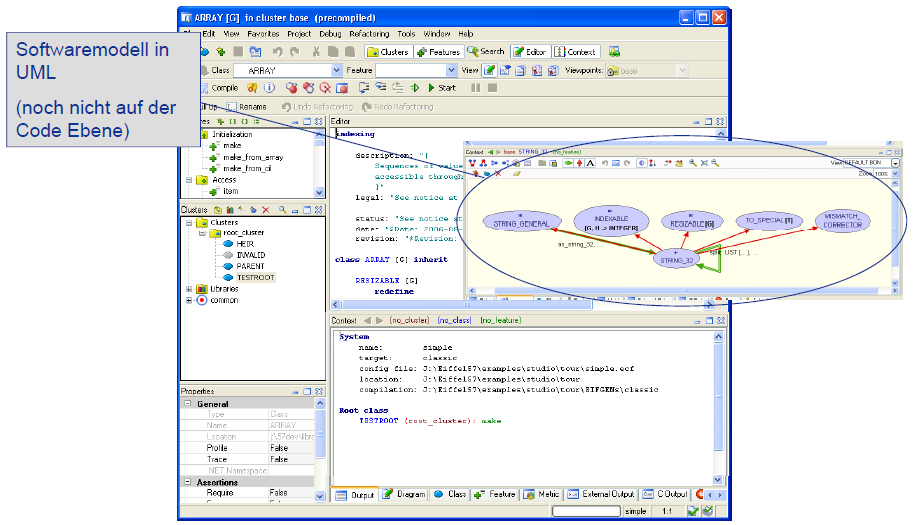
\includegraphics[scale=0.5]{UpperCASE.png}\\
%		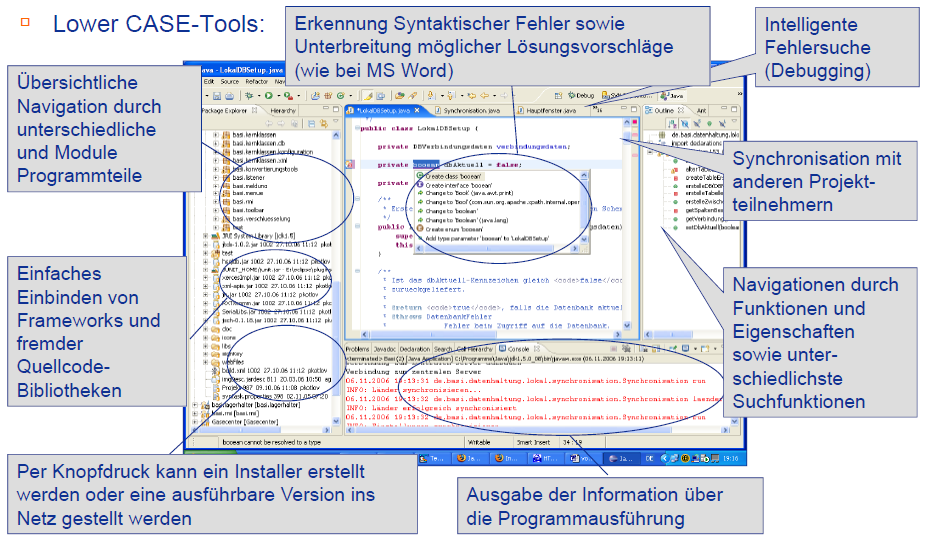
\includegraphics[scale=0.5]{LowerCASE.png}
\end{enumerate}
%
%\newpage
%
%\begin{enumerate}
%	\item Nennen Sie die Abschnitte eines typischen Produktlebenszyklus.
%	\item Welche Prozesse finden in den einzelnen Phasen eines Produktlebenszyklus statt?
%		\begin{itemize}
%			\item Anforderungen
%				\begin{itemize}
%					\item Anforderungsanalyse
%					\item Anforderungserfassung
%				\end{itemize}
%			\item Produktplanung
%				\begin{itemize}
%					\item Programm-/Portfolio-Planung
%					\item Projektplan-, Team- \& Kosten-Festlegung
%				\end{itemize}
%			\item Entwicklung
%				\begin{itemize}
%					\item Mechanische Konstruktion
%					\item Elektrokonstruktion
%					\item Softwareentwicklung
%					\item Simulation, DMU/PMU
%					\item Absicherung/Versuche
%					\item Dokumentation
%				\end{itemize}
%			\item Prozessplanung
%				\begin{itemize}
%					\item Prozessplanung
%					\item Analgenplanung
%					\item Anlagenentwicklung
%					\item Einkauf
%					\item Simulation/Versuche
%				\end{itemize}
%			\item Produktion
%				\begin{itemize}
%					\item Herstellung
%					\item Zusammenbau
%					\item Qualitätssicherung
%				\end{itemize}
%			\item Betrieb
%				\begin{itemize}
%					\item Vertrieb
%					\item Service
%					\item Wartung und Reparatur
%				\end{itemize}
%			\item Recycling
%				\begin{itemize}
%					\item Recycling
%				\end{itemize}
%		\end{itemize}
%	\item Warum sollten die Entwicklungszeiten möglichst kurz sein?
%	\item Welchen Einfluss hat die Produktkomplexität auf die Produktentwicklung?
%	\item Warum spielt die frühe Phase in der Produktentwicklung eine entscheidende Rolle?
%	\item Nennen Sie Anforderungen an einen effizienten Produktentwicklungsprozess.
%	\item Nennen Sie die Schritte in einem Entwicklungsprozess nach VDI 2221.
%	\item Was versteht man unter virtueller Produktentwicklung?
%	\item Wie werden die Entwicklungsstufen der rechnergestützten Produktentwicklung unterschieden?
%	\item Benennen Sie folgende Begriffe: CAD, E-CAD, CAE, CASE, CAT, MKS, FEM, CFD, VR, CAM, TPD, PDM, HIL, SIL, PLM, PLC, STEP, IGES, DMU, VMU, CAS, PPC, RC, NC, MC
%	\item Was sind und wofür werden digitale Produktmodelle / digitale Prozessmodelle verwendet?
%	\item Was ist Frontloading? Wie / warum wird es eingesetzt?
%	\item Was ist Simultaneous Engineering? Wie / warum wird es eingesetzt?
%	\item Was versteht man unter einem "Development Process" und einem "Development Workflow"?
%	\item Wodurch unterscheiden sich ein "Development Process" und ein "Development Workflow"?
%	\item Was ist der Unterschied zwischen einem DUM und einem VMU?
%	\item Was versteht man unter einem horizontalen und einem vertikalen Datentransfer in Bezug auf die computergestützte Entwicklung mechatronischer Produkte?
%	\item Nennen Sie Formate für den Austausch von Geometriedaten in CAx-Workflows.
%	\item Erklären Sie die folgenden Begriffe in Bezug auf den Datenaustausch in CAx-Workflows: Integrität, Datenkonsistenz, Datenrobustheit, Kompatibilität.
%	\item Was versteht man unter einem Produktmodell im Sinne der computergestützten Entwicklung?
%	\item Nennen Sie Beispiele für hardwarebasierte und virtuelle Produktmodelle.
%	\item Erklären Sie die Begriffe "physikalische Modellbildung" und "phänomenologische Modellbildung".
%	\item Vergleichen Sie die Vorteile von computergestützter Simulation und hardware-basierter Entwicklung.
%	\item Welche Verfahren zur Modellbildung werden bei folgenden Computer-gestützten Simulationsverfahren angewandt: FEM, MKS (MBS), 3D-CFD
%	\item Nennen Sie Anwendungen in der Entwicklung mechatronischer Produkte für folgende computergestützte Simulationsverfahren: FEM, MKS (MBS), CFD
%	\item Nennen Sie mind. 5 Beispiele für CAx-Workflows.
%	\item Beschreiben Sie folgende CAx-Workflows: CAD – DMU, CAD – FEM, CAD – MKS (MBS).
%	\item Was versteht man unter den Begriffen "Tesselierung" und "Meshing".
%	\item Nennen Sie die Funktionalitäten von PDM-Systemen (jeweils Produkt-bezogen und Prozessbezogen).
%	\item Erklären Sie die fünf Hauptfunktionalitäten von PDM-Systemen näher.
%	\item Was versteht man unter Produktdaten (im Sinne der virtuellen Produktentwicklung)?
%	\item Erklären Sie eine möglich Abfolge von Schritten bei der Änderung eines mechatronischen Produktes.
%	\item Wie ist ein PDM-System generell aufgebaut?
%	\item Was versteht man unter dem Begriff "Mechatronik"?
%	\item Welche Disziplinen sind in die Entwicklung mechatronischer Produkte involviert?
%	\item Was sind die Herausforderungen bei der Entwicklung mechatronischer Produkte im Vergleich mit konventionellen mechanischen Produkten?
%	\item Erklären Sie einen beispielhaften Entwicklungsprozess mechatronischer Produkte anhand des V-Modells.
%	\item Welche Komponenten beinhalten mechatronische Systeme? Wie sind diese Komponenten die verschiedenen Domänen zuzuordnen?
%	\item Was sind Aktuatoren?
%	\item Welche Arten von Aktuatoren gibt es?
%	\item Was sind Sensoren?
%	\item Welche Arten von Sensoren gibt es?
%	\item Nenne Sie Anforderungen an Sensoren in mechatronischen Produkten.
%	\item Nennen Sie Verfahren zur Weg- bzw. Winkelmessung bei mechatronischen Produkten.
%	\item Was versteht man unter Signalverarbeitung in mechatronischen Produkten?
%	\item Was versteht man unter Prozessdatenverarbeitung in mechatronischen Produkten?
%	\item Was versteht man unter Echtzeitdatenverarbeitung in mechatronischen Produkten?
%	\item Was versteht man unter "Hardware-in-the-Loop" Entwicklung?
%	\item Was ist ein HIL-Simulator?
%	\item Warum wird HIL angewandt? Wo sind die Vor- bzw. Nachteile dieser Entwicklungsmethode?
%	\item Was versteht man unter "Software-in-the-Loop" Entwicklung?
%	\item Warum wird SIL angewandt? Wo sind die Vor- bzw. Nachteile dieser Entwicklungsmethode?
%	\item Was sind "Upper-CASE-Tools” bzw. "Lower-CASE-Tools”?
%	\item Nennen Sie Anwendungsbeispiele für E-CAD.
%	\item Skizzieren Beispielhaft ein mechatronisches System und beschreiben Sie die Komponenten und Funktionen.
%	\item Erklären Sie den Unterschied zwischen steuern und regeln.
%	\item Was versteht man unter CAE?
%	\item Skizzieren Sie eine beispielhafte Prozesskette CAD-CAE und benennen Sie die Workflows und Datenflüsse.
%	\item Was versteht man unter FEM? Wozu wird diese Methode eingesetzt?
%	\item Worauf ist bei der Aufbereitung von Geometriedaten für die FEM-Simulation besonders zu achten?
%	\item Was versteht man unter "Diskretisierung" in der Strukturmechanik?
%\end{enumerate}
\end{document}
